% Body of the EG 2027 short paper (issue #97). Numbers come from committed summary counts:
% report/data/bowser/numbers.csv (hand-checked build, 2026-11-03) and the no-hand-input
% rebuild of lowpoly #93 (papercraft data/bowser-fresh/comparison.md, 2026-11-04).
% No figure shows the template's pages or pieces (personal-use terms); all drawings are ours.

\begin{figure*}[t]
\centering
\begin{tikzpicture}[
  node distance=2.6mm,
  box/.style={draw, rounded corners=2pt, align=center, font=\footnotesize, minimum height=9mm,
              text width=19.5mm, fill=#1},
  box/.default=white,
  arr/.style={-{Stealth[length=2mm]}, thick},
  lab/.style={font=\scriptsize, align=center, text=black!70}]
  \node[box=black!5]  (pdf)  {PDF template\\+ model YAML};
  \node[box, right=of pdf]  (ren)  {Render\\\texttt{pdftoppm}};
  \node[box, right=of ren]  (det)  {Separate ink;\\pieces, folds\\(Alg.~\ref{alg:pieces})};
  \node[box, right=of det]  (ocr)  {Read numbers,\\pair up\\(Alg.~\ref{alg:read})};
  \node[box, right=of ocr]  (twin) {Mirror twins:\\predict, repair\\(Alg.~\ref{alg:twins})};
  \node[box, right=of twin] (chk)  {Self-checks,\\3D fold-up};
  \node[box=black!5, right=of chk] (svg) {Layered SVG:\\Cut / Score / Draw};
  \node[box=orange!12, below=6mm of twin, text width=30mm] (ask) {Check page: only\\open questions};
  \foreach \a/\b in {pdf/ren, ren/det, det/ocr, ocr/twin, twin/chk, chk/svg} \draw[arr] (\a) -- (\b);
  \draw[arr] (chk.south) |- (ask.east);
  \draw[arr] (ask.west) -| node[lab, pos=0.75, left] {answers,\\digit samples} (ocr.south);
\end{tikzpicture}
\caption{Pipeline. Every stage after rendering works in millimetres on our own representation.
The constraints of Section~\ref{sec:constraints} are applied automatically; a person sees only
what they cannot settle, and every answer is replayed on later builds and teaches the digit
reader.}
\label{fig:pipeline}
\end{figure*}

\section{Introduction}

Papercraft masks and helmets made of low-poly cardstock are distributed by their designers,
for sale or free for personal use, as PDF templates made for a home printer and scissors. Each
page holds unfolded pieces drawn with three kinds of ink: solid cut lines, dashed (valley) and
dash-dot (mountain) fold lines, and small edge numbers. Two edges that carry the same number
are glued together, one of them through a tab. Many builders now own a cutting machine that can
cut, score and draw on cardstock, but it needs vector paths assigned to those operations, and the
template is a picture.

Raster-to-vector methods are judged by how close the result looks to the input
\cite{selinger2003potrace,hilaire2006,noris2013,bessmeltsev2019,egiazarian2020}. For a template
this is the wrong measure. A fold traced as dashes becomes a row of cuts that perforate the piece;
a missed corner moves a cut by a millimetre that no one sees but that keeps a seam from
closing; and an edge number misread as a near-identical one sends the builder to the wrong piece.
None of these errors changes the picture much.

Our observation is that a template is heavily redundant, and the redundancy can be checked
without ground truth. Every edge number appears exactly twice, on two edges of equal length, one
of which ends at a tab fold. Most pieces of a mask have a mirror twin with the same face. And the
pieces, folded at their fold lines and glued at their numbers, must close into one surface. We
build a vectorization pipeline (Figure~\ref{fig:pipeline}) that uses these constraints in three
ways: to choose between uncertain readings, to repair traced geometry, and to reduce human
review to the cases the constraints leave open. Our contributions are:
\begin{itemize}\setlength\itemsep{0pt}
\item an ink-separation and polygon-fitting method for low-poly templates that produces cut
  polygons, single straight fold lines and OCR'd edge numbers instead of traced strokes;
\item a two-reader number reader whose uncertain readings are resolved jointly by the pairing
  constraint;
\item mirror-twin matching by sequence alignment of edge lengths, used to predict numbers, add
  missing folds and average corners;
\item an evaluation on one 21-sheet template, with and without human answers.
\end{itemize}
The software is open source \codelink. Our test case is a template found online, free for
personal use and no longer maintained, whose small, low-quality edge numbers are hard to read by eye;
the pipeline recovers them, and its 3D fold-up doubles as an interactive view of where each piece
goes.

\section{Related work}

General vectorizers trace strokes or regions: Potrace fits curves to bitmap
boundaries \cite{selinger2003potrace}, contour following \cite{suzuki1985} with
Douglas--Peucker simplification \cite{douglas1973} gives polygons, and line-drawing
vectorization recovers stroke topology \cite{hilaire2006,noris2013,bessmeltsev2019}, also with
learning on technical drawings \cite{egiazarian2020}. Differentiable and generative
vectorizers \cite{li2020diffvg,ma2022live,rodriguez2023starvector} optimise visual similarity.
None of them assigns fabrication meaning (cut versus fold, which edges glue) or checks it. Text
in drawings is usually read by an OCR engine such as Tesseract \cite{smith2007tesseract}; we add
a page-trained digit matcher and a joint decision. Papercraft research mostly goes the other
way, from a mesh to an unfolding \cite{mitani2004,takahashi2011}; we recover the unfolding's
pieces and gluing from print. Our mirror matching is a 2D, combinatorial cousin of symmetry
detection on shapes \cite{mitra2006symmetry}, using sequence alignment \cite{needleman1970}
and a least-squares similarity fit \cite{umeyama1991}.

\section{Method}
\label{sec:method}

The input is the PDF and a short YAML file per model that names the pages, the cardstock colour
of each page and the template's fold styles. Pages are rendered at 180\,dpi with
\texttt{pdftoppm}; all geometry below is converted to millimetres with the page's own scale.

\subsection{Pieces, cut polygons and folds}

Printed ink is split by darkness and extent (Algorithm~\ref{alg:pieces}). Connected components
longer than 4.3\,mm are cut lines; dark short components are number glyphs; the remaining
ink is fold dashes. A piece is what a flood fill of the paper from the page border cannot reach,
which keeps numbers and dashes touching a cut from carving notches into it. Pieces may touch at a
corner, so every enclosed open area seeds its own piece and grows through the cut ink.

Because the model is low-poly, a cut outline is a polygon with no curves. The contour is
simplified, small bumps where a number touches a straight cut are removed, and each edge is
refitted as a robust straight line through the printed cut ink near it, so that the edge follows
the line, not the border of the filled region. Corners move to where neighbouring fitted lines
meet, and vertices where the outline turns less than $4^\circ$ are dropped.

Fold dashes inside a piece are found with a probabilistic Hough transform, merged when collinear
(numbers printed on a fold interrupt its dashes), refitted to the dash pixels, and then
stretched from the fold's midpoint to the first cut edge in each direction, snapping to a corner
within 1.5\,mm. A stretched fold must still be at least 60\,\% dashes, which rejects lines
across a fan of folds. The fold's style is read from its dash runs: a dash-dot line has long
runs where the dot merges with a dash. Each glyph group becomes a number mark attached to the
nearest cut edge or fold it labels; a number on a fold marks a tab (Figure~\ref{fig:piece}).

\begin{algorithm}[t]
\caption{Pieces, cut polygons and folds of one page}
\label{alg:pieces}
\begin{algorithmic}[1]
\Require page raster $I$, scale $s$ (mm/px)
\Ensure pieces $P$: cut polygon, folds, number marks
\State $C, G, D \gets$ \Call{SplitInk}{$I$} \Comm{cut, glyph, dash masks}
\State $O \gets$ \Call{FloodFill}{$\neg\,\mathrm{close}(C)$, border} \Comm{paper outside}
\For{each enclosed region $R$ of $\neg O$}
  \State $Q \gets$ \Call{ApproxPoly}{contour$(R)$, 1.5\,px}
  \State $Q \gets$ \Call{Straighten}{$Q$} \Comm{drop bumps from numbers}
  \Repeat
    \State fit each edge of $Q$ to $C$ ink within a band (Huber)
    \State move each corner to its two fitted lines' intersection
    \State replace runs of $\le 3$ vertices whose edges leave $C$
  \Until{no change}
  \State drop vertices turning $< 4^\circ$; merge edges $< 0.8$\,mm
  \State $F \gets$ \Call{HoughSegments}{$D \cap R$}; merge collinear
  \For{each $f \in F$}
    \State extend $f$ to the cut on both sides; snap ends to corners
    \State \textbf{if} dash coverage$(f) < 0.6$ \textbf{then} discard $f$
    \State style$(f) \gets$ dashed or dash-dot from its run lengths
  \EndFor
  \State $P \gets P \cup \{(Q, F)\}$
\EndFor
\State group $G$ into number marks; attach each to the nearest edge or fold
\end{algorithmic}
\end{algorithm}


\begin{figure}[t]
\centering
\begin{tikzpicture}[scale=0.55, font=\scriptsize,
  cut/.style={very thick}, fold/.style={thick, dashed, black!60},
  score/.style={thick, blue!70!black}, num/.style={fill=white, inner sep=0.5pt}]
  % (a) as printed: piece A with a tab, dashed folds and numbers
  \begin{scope}
    \draw[cut] (0,0) -- (3,0) -- (3.6,1.8) -- (3,2.2) -- (2.2,3.4) -- (0.3,2.6);
    \draw[cut] (0,0) -- (-0.7,0.4) -- (-0.5,2.2) -- (0.3,2.6);  % tab
    \foreach \t in {0.05,0.17,...,0.95} \draw[fold] ($(0,0)!\t!(0.3,2.6)$) -- ($(0,0)!\t+0.06!(0.3,2.6)$);
    \foreach \t in {0.05,0.17,...,0.95} \draw[fold] ($(3,0)!\t!(0.3,2.6)$) -- ($(3,0)!\t+0.06!(0.3,2.6)$);
    \node[num, rotate=84] at (-0.15,1.3) {214};
    \node[num] at (1.5,-0.25) {131};
    \node[num, rotate=56] at (2.75,2.95) {088};
    \node at (1.6,-0.9) {(a) printed};
  \end{scope}
  % (b) vectorised: cut polygon, one score line per fold, numbers as text
  \begin{scope}[xshift=5.2cm]
    \draw[cut] (0,0) -- (3,0) -- (3.6,1.8) -- (3,2.2) -- (2.2,3.4) -- (0.3,2.6) -- (-0.5,2.2) -- (-0.7,0.4) -- cycle;
    \draw[score] (0,0) -- (0.3,2.6);
    \draw[score] (3,0) -- (0.3,2.6);
    \node[num, text=red!70!black] at (-0.15,1.3) {214};
    \node[num, text=red!70!black] at (1.5,-0.25) {131};
    \node[num, text=red!70!black] at (2.75,2.95) {088};
    \node at (1.4,-0.9) {(b) Cut / Score / Draw};
  \end{scope}
  % (c) mirror twin: same face lengths walked the other way
  \begin{scope}[xshift=13.3cm, xscale=-1]
    \draw[cut] (3.6,1.8) -- (3,2.2) -- (2.2,3.4) -- (0.3,2.6) -- (0,0) -- (3,0);
    \draw[cut] (3,0) -- (3.4,-0.6) -- (3.9,1.2) -- (3.6,1.8); % tab elsewhere
    \draw[score] (3,0) -- (0.3,2.6);
    \draw[score] (3,0) -- (3.6,1.8);
    \node[num] at (1.5,-0.25) {132};
    \node[num, rotate=-56] at (2.75,2.95) {089};
    \node[num, rotate=-84] at (-0.15,1.3) {215};
    \node at (1.6,-0.9) {(c) twin $A'$};
  \end{scope}
\end{tikzpicture}
\caption{A schematic piece (our drawing, not from the template). (a) Printed ink: solid cut,
dashed folds, edge numbers; the number on a fold marks a tab. (b) Vector result: one cut polygon,
one straight score line per fold, numbers as text. (c) Its mirror twin: the numbered lines have
the same lengths in reverse order, while the tab may sit on another edge.}
\label{fig:piece}
\end{figure}

\subsection{Reading the edge numbers}

Numbers are read, never traced. Each mark is rotated upright along its edge and read by two
readers (Algorithm~\ref{alg:read}). Tesseract \cite{smith2007tesseract} reads it as one line of
digits in both orientations. A digit matcher is trained on the page itself: marks Tesseract
reads with confidence $\ge 90$ are split into digit cells, and every digit a person has corrected
is added. A reading is accepted when both readers agree or Tesseract alone has confidence $\ge 93$.

The remaining marks are decided together. Since every number must appear exactly twice, an
uncertain mark, taken in order of the matcher's confidence, prefers a reading close to its best
score that completes a pair, then one that starts a pair. It is trusted only when the completing
reading was ranked first by one of the two readers.

\begin{algorithm}[t]
\caption{Two readers and joint pair-up}
\label{alg:read}
\begin{algorithmic}[1]
\Require number marks $M$, hand answers $H$
\Ensure text and trust for every $m \in M$
\For{$m \in M$} $(t_m, c_m) \gets$ best Tesseract read over $0^\circ, 180^\circ$ \EndFor
\State train matcher on digits of $\{m : c_m \ge 90\} \cup H$
\For{$m \in M$}
  \State $K_m \gets$ matcher candidates (text, score), best first
  \If{$m \in H$} accept $H_m$
  \ElsIf{$t_m = K_m[1]$ \textbf{or} $c_m \ge 93$} accept $t_m$
  \EndIf
\EndFor
\State $n(x) \gets$ number of accepted marks reading $x$
\For{undecided $m$ by decreasing best score}
  \State $A \gets \{k \in K_m : \mathrm{score}(k) \ge \mathrm{score}(K_m[1]) - 0.05\}$
  \State $x \gets$ first $k \in A$ with $n(k)=1$, else with $n(k)=0$, else $K_m[1]$
  \State trust$(m) \gets [\,n(x)=1 \wedge x \in \{K_m[1], t_m\}\,]$; $n(x)$ += 1
\EndFor
\State flag every $m$ whose text $x$ has $n(x) \ne 2$
\end{algorithmic}
\end{algorithm}

\subsection{Constraints that check the trace}
\label{sec:constraints}

\paragraph{Pairing.} Every number now gets one status from its two copies: \emph{ok} (one plain
edge and one tab, lengths within 1\,mm), \emph{unpaired}, \emph{length mismatch}, \emph{no tab},
\emph{both tabs} or \emph{extra copy}. An unpaired number is matched to an unpaired line of the
same length on the other side only when the reader offered that number as an alternative or the
two differ in one digit, and no other candidate exists.

\paragraph{Mirror twins.} A mask is mirror-symmetric, so most pieces have a twin cut from the
same cardstock (Algorithm~\ref{alg:twins}). Walking round one piece, the lengths of its numbered
lines read the same as its twin's walked the other way, with gaps where a number found no line
or a tab sits elsewhere. We align the two cyclic length sequences with a Needleman--Wunsch style
recurrence \cite{needleman1970} over all cyclic shifts, and accept a twin when at least 70\,\% of
the lines agree within 1\,mm. Twins are taken greedily by agreement. Matched line midpoints give
a similarity transform with reflection \cite{umeyama1991} that lays one twin on the other.
Twins then give three checks and repairs: a line and its mirror line should be equally long; a
fold of one twin with no fold at the mirrored place on the other is a missed fold, added in the
style printed under it; and glue pairs mirror, so if line $a$ of piece $A$ glues to piece $C$,
the mirror of $a$ on $A$'s twin glues to $C$'s twin, which predicts its number. Mirror corners
of the face that lie 0.2--1.5\,mm apart both move to their mirrored mean; tab corners find no
partner and stay, since a twin's tabs may sit on other edges.

\begin{algorithm}[t]
\caption{Mirror twins: matching, prediction, repair}
\label{alg:twins}
\begin{algorithmic}[1]
\Require pieces with cut polygons, folds, numbered lines
\For{pairs $(A,B)$, same cardstock, perimeters within 25\,\%}
  \State $\ell_A \gets$ lengths of numbered lines of $A$ in walking order
  \State $\ell_B \gets$ same for $B$, \emph{reversed}
  \State $(\sigma, \pi) \gets \max_k$ \Call{Align}{$\ell_A$, roll$(\ell_B, k)$}
  \Statex \Comm{gain 2 if $|\Delta| \le 1$\,mm, 1 if $\le 3$\,mm}
  \State keep $(A,B,\pi)$ if share of agreeing lines $\ge 0.7$
\EndFor
\State choose twins greedily by share, each piece at most once
\For{each twin $(A,B,\pi)$}
  \State $T \gets$ similarity with reflection fit on matched midpoints
  \State flag line pairs in $\pi$ differing $> 1$\,mm in length
  \State add folds of $A$ missing at $T(\cdot)$ on $B$, and vice versa
  \State move mutual-nearest corners 0.2--1.5\,mm apart to their mean
  \For{unpaired line $a$ of $A$ with mirror $b=\pi(a)$ on $B$}
    \If{$b$ glues cleanly to $c$ on $C$ and $C$ has twin $C'$}
      \State predict number of $a$ := number on $\pi_{CC'}(c)$
    \EndIf
  \EndFor
\EndFor
\end{algorithmic}
\end{algorithm}

\paragraph{Self-checks and fold-up.} Further checks need no ground truth: a fold that meets the
cut between two corners (a missed corner), cut ink that runs past a traced corner (a clipped
corner), a piece traced twice, and a page whose glued pairs are all slightly too long or short
(a scale error). The strongest check folds every piece at its fold lines into a 3D mesh, glues
each numbered pair and measures the gap left; a misread number or a mistraced line shows up as a
glue that does not close.

\paragraph{Human answers.} What the constraints cannot settle is shown on a local check page as
cards with the scan around both copies of a number and the traced lines. Answers are saved as
CSV files (number corrections, hand-drawn lines, piece edits) that every later build applies
before the constraints run, and each corrected number teaches the digit matcher.

\subsection{Output}

The result is one Inkscape SVG per model, with one layer per cardstock colour and one group per
piece. Each group holds a \emph{Cut} path (the polygon, tabs included), a \emph{Score} group with
one straight line per fold, split by valley and mountain style as the YAML names them, and a
\emph{Draw} group with the edge numbers as text. Ink outside every piece stays on a hidden
\emph{Review} layer, so nothing disappears silently. An export step converts to inches for the
cutting machine's software and replaces the template's three-digit numbers by short labels.

\section{Results}

We ran the pipeline on one low-poly mask template, free for personal use
\cite{papercraftcat2017}: 24 US Letter pages, 21 of them with pieces on six cardstock colours.
Table~\ref{tab:results} compares the run with no human input to the build after all answers.
Shapes are good without help: the unsupervised cut outlines lie a median 0.60\,mm from the
checked ones, 90\,\% within 1.4\,mm, and only 3 of 178 pieces are more than 3\,mm off. Mirror
averaging alone made 262 corner moves and added 10 folds. The numbers are the bottleneck: the
unsupervised run pairs 1059 of 1575 numbers with the right partner, 10 with a wrong one, and
leaves 496 open, most of them tab-versus-edge confusions and misreads.


\begin{figure}[t]
\centering
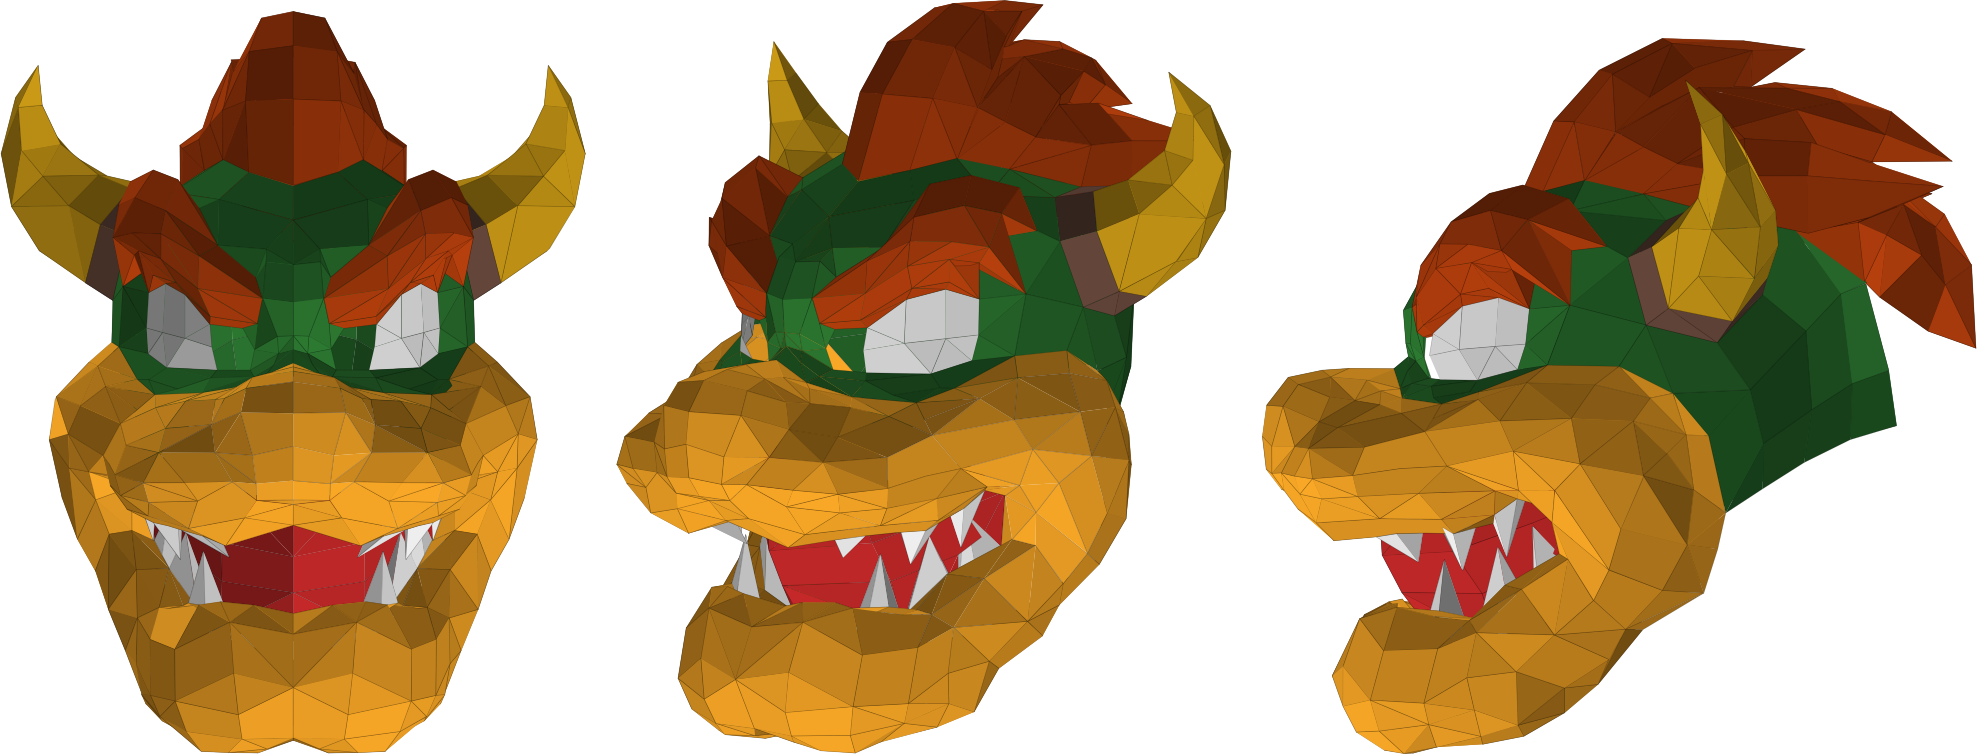
\includegraphics[height=2.6cm]{figures/mask.png}
\caption{The reconstructed mask: our pieces, folded at their score lines and glued at their
recovered numbers (front, three-quarter and side view, cardstock colours from the model YAML).
All 754 glued edges close. The same fold-up drives an interactive viewer that links each 3D face
to its flat piece. Bowser is a Nintendo character (\emph{Super Mario}). Mask design: Papercraft Cat (Remy Del Toro) \cite{papercraftcat2017}.}
\label{fig:mask}
\end{figure}

\begin{table}[t]
\centering\footnotesize
\caption{One 21-sheet template, without and with human answers.}
\label{tab:results}
\begin{tabular}{@{}lrr@{}}
\toprule
 & no answers & all answers \\
\midrule
edge numbers found            & 1575 & 1569 \\
\quad trusted reads           & 970  & 1487 \\
\quad paired with right piece & 1059 & 1548 \\
\quad paired with wrong piece & 10   & 0 \\
\quad open                    & 496  & 21 \\
mirror twin pairs             & 86   & 89 \\
3D fold-up: glues closing     & 527 / 631 & 754 / 754 \\
3D fold-up: connected parts   & 3    & 1 \\
\midrule
human input (rows)            & 0    & 1079 \\
\quad number answers (changed) & --  & 670 (14) \\
\quad hand-drawn lines         & --  & 90 \\
\quad piece edits              & --  & 319 \\
\bottomrule
\end{tabular}
\end{table}

With all answers, 1548 of 1569 numbers pair cleanly and every one of the 754 glued edges closes
in the fold-up, with a median gap of 0.1\,mm (Figure~\ref{fig:mask}). Of the 21 numbers left open, 6 are numbered edges
around an eye opening that glue to nothing; the others are length mismatches and extra copies
that do not keep the fold-up from closing. Of the 670 number
answers only 14 changed the reading of the day, but they were not redundant: a reader trained
without them reads 299 of the same marks differently. Replaying the answers in rounds of 100,
least-trusted first, fixes about one pair per answer (1059, 1154, 1252, 1326, 1400 pairs after
0--400 answers), so roughly 550 answers would rebuild the checked result from scratch, half the
1079 rows the first build needed. An ablation of the automatic repairs is a warning: a third of
the fixes applied without asking in the unsupervised run were wrong (38 of 112), so an automatic
fix should need a second signal, a twin or the fold-up, and otherwise be shown as a suggestion.

\section{Limitations and future work}

The evaluation covers one template from one designer; other
line styles need other thresholds in the YAML, and a multi-template benchmark with synthetic
ground truth is in preparation. Reading is the weak stage. The 1548 confirmed numbers are a
labelled set for the digit matcher, and a matcher trained on them should shorten the open list
for the next template by the same designer; measuring this needs held-out pages. Asking
about whole glue pairs proposed by the fold-up would settle two numbers with one answer.

The vector model makes changes possible that a printed template does not allow: wider glue
tabs for the builder's adhesive, a different paper size, recolouring, re-segmenting the folded
mesh into fewer pieces, and nesting the pieces on the fewest sheets. These are the subject of
an extended paper; here we have shown that the template itself can be read reliably, because
it checks itself.
